\begin{abstract}
The Mars Science Laboratory's Curiosity rover has been instrumental in studying Mars' geology and potential habitability through its ChemCam instrument, which uses Laser-Induced Breakdown Spectroscopy (LIBS) for elemental quantification.
However, the computational interpretation of LIBS data faces challenges such as multicollinearity and matrix effects, complicating the accurate prediction of elemental compositions.
This study aims to scrutinize the limitations of the existing Multivariate Oxide Composition (MOC) model, used for predicting major oxides in Martian geological samples based on Earth-based calibration data.
We propose ...
Enhancing the MOC model's predictive accuracy could significantly advance the scientific objectives of the Mars Science Laboratory mission by providing more precise insights into Martian geology and habitability.
\end{abstract}

% Acknowledgments
% - Acknowledge any contributions, support, or guidance from individuals, organizations, or institutions.

\section{Introduction}\label{sec:introduction}
NASA has been studying the Martian environment for decades through a series of missions, including the Viking missions~\cite{marsnasagov_vikings}, the \gls{mer} mission~\cite{marsnasagov_observer, marsnasagov_spirit_opportunity}, and the \gls{msl} mission~\cite{marsnasagov_msl}, each building on the knowledge gained from the previous ones.
Today, the rovers exploring Mars are equipped with sophisticated instruments for analyzing the chemical composition of Martian soil in search of past life and habitable environments.

Part of this research is facilitated through interpretation of spectral data gathered by \gls{libs} instruments, which fire a high-powered laser at soil samples to create a plasma.
The emitted light is captured by spectrometers and analyzed using machine learning models to assess the presence and concentration of certain major oxides, informing NASA's understanding of Mars' geology~\cite{cleggRecalibrationMarsScience2017}.

However, predicting major oxide compositions from \gls{libs} data still presents significant computational challenges.
These include the high dimensionality and non-linearity of the data, compounded by issues of multicollinearity and matrix effects~\cite{andersonImprovedAccuracyQuantitative2017}.
Such effects can cause the intensity of emission lines from an element to vary independently of that element's concentration, introducing unknown variables that complicate the analysis.
Furthermore, the high cost of data collection often results in small datasets, exacerbating the difficulty of building accurate and robust models.

Previous work has aimed to improve the prediction of major oxide compositions from \gls{libs} data by using regression techniques and dimensionality reduction with feature selection.
These methods have been used to enhance both the accuracy and interpretability of the prediction models.
Tailored approaches have also been developed, where different models are selected based on their performance with specific spectral characteristics~\cite{rezaei_dimensionality_reduction, andersonPostlandingMajorElement2022}.
Moreover, models incorporating physical principles have demonstrated improved accuracy by handling residuals that traditional models fail to explain~\cite{song_DF-K-ELM}.
However, predicting oxide compositions remains challenging due to the complex, nonlinear nature of \gls{libs} data.
This underscores the need for continued research into more adaptive and robust machine learning strategies to tackle these issues effectively.

This thesis aims to improve upon previous work in the field of \gls{libs} data analysis.
Our goal is to develop a machine learning pipeline that is tailored to the unique characteristics of \gls{libs} data, with the goal of achieving higher prediction accuracy and robustness.

To achieve these objectives, we build upon the baseline established in~\cite{p9_paper} and systematically explore ten different machine learning models. 
These models were identified and selected through a combination of extensive literature review and the consideration of unconventional approaches not typically covered in the \gls{libs}-based calibration literature.
The ten models fall into three categories: Ensemble learning models, linear and regularization models, and neural network models.
In addition to model exploration, we also investigate a selection of preprocessing techniques: scaling (including normalization), dimensionality reduction, and data transformation.
Specifically, we designed and implemented a framework for experimental analysis using the automated hyperparameter optimization framework Optuna~\cite{optuna_2019}.
We then used this framework to determine the most effective combinations of preprocessing methods and models for each regression target.
We began by identifying the most promising models from the literature, after which we evaluated various preprocessing techniques to understand their impact on model performance, selecting those that demonstrated the highest impact on improving the performance of each model.
Following preprocessing, we optimized the chosen models through hyperparameter tuning to ensure optimal performance tailored to the specific data characteristics of each oxide.
Once the best hyperparameters were identified, a stacking ensemble method was employed to create a meta learner for each oxide, significantly enhancing prediction accuracy and robustness beyond the capabilities of individual models.
% TODO: Superior performance needs to be replaced with actual numbers
Through extensive experiments on \gls{libs} data, we systematically assessed and demonstrated the superior performance of our approach compared to existing methods, focusing on significant improvements in prediction accuracy and robustness.

Our key contributions are as follows:
\begin{itemize}
    \item We develop a novel machine learning pipeline that demonstrates improved accuracy and robustness in predicting major oxide compositions in \gls{libs} data.
    \item We have developed a novel optimization approach and tool for tuning and evaluating machine learning models along with preprocessing techniques, providing a systematic and efficient method for selecting the best configuration.
    \item By outperforming existing methods, our approach has established new benchmarks for accuracy and robustness in \gls{libs} data analysis.
\end{itemize}


% TODO: Add remaining sections
The remainder of this paper is organized as follows:
Section~\ref{sec:background} provides background on the onoging Mars exploration missions, the \gls{libs} technique, and the baseline \gls{moc} model.
Section~\ref{sec:problem_definition} formally defines the problem addressed in this work.
Section~\ref{sec:methodology} describes our proposed methodology, including data preprocessing, dimensionality reduction, and machine learning models.
Section~\ref{sec:experiments} presents our experimental setup and results.
Finally, Section~\ref{sec:conclusion} concludes the paper and discusses future work.

In table \ref{tab:terms}, we provide a list of terms used throughout this paper.

\begin{table}
\centering
\begin{tabularx}{\columnwidth}{lX} % l for left, X for the cell that should be wrapped
\toprule
Term & Definition \\
\midrule
Sample & A physical specimen of rock, soil, or other material collected for scientific analysis.\\
Location & The specific point on a sample where a LIBS laser is targeted. There are typically multiple locations per sample. \\ 
Target & Refers to the variable that a machine learning model is trained to predict. \\
\bottomrule
\end{tabularx}  
\caption{Table of Terms}
\label{tab:terms}
\end{table}
\section{Background}\label{sec:background}
\subsection{Preprocessing}

\subsubsection{Standard Scaler}

\subsubsection{Max Absolute Scaler}

\subsubsection{MinMax Scaler}

\subsubsection{Robust Scaler}

\subsubsection{Norm 3}
As previously mentioned, the \gls{chemcam} instrument consists of three spectrometers, each producing 2048 channels.
For data normalization, we follow the approach taken by the SuperCam team and normalize across individual spectrometers' wavelength ranges, a process known as \textit{Norm 3}~\cite{andersonPostlandingMajorElement2022}.
This method ensures that the wavelength intensities captured by each spectrometer is normalized independently.

Figure~\ref{fig:spectral_plot} shows a spectral plot of the \gls{ccs} data for the \textit{ultramafic} sample, illustrating the three distinct spectral regions, each captured by one of the three spectrometers. Specifically, one spectrometer captures the \gls{uv} region, another captures the \gls{vio} region, and the third captures the \gls{vnir} region.

\begin{figure}[H]
	\centering
	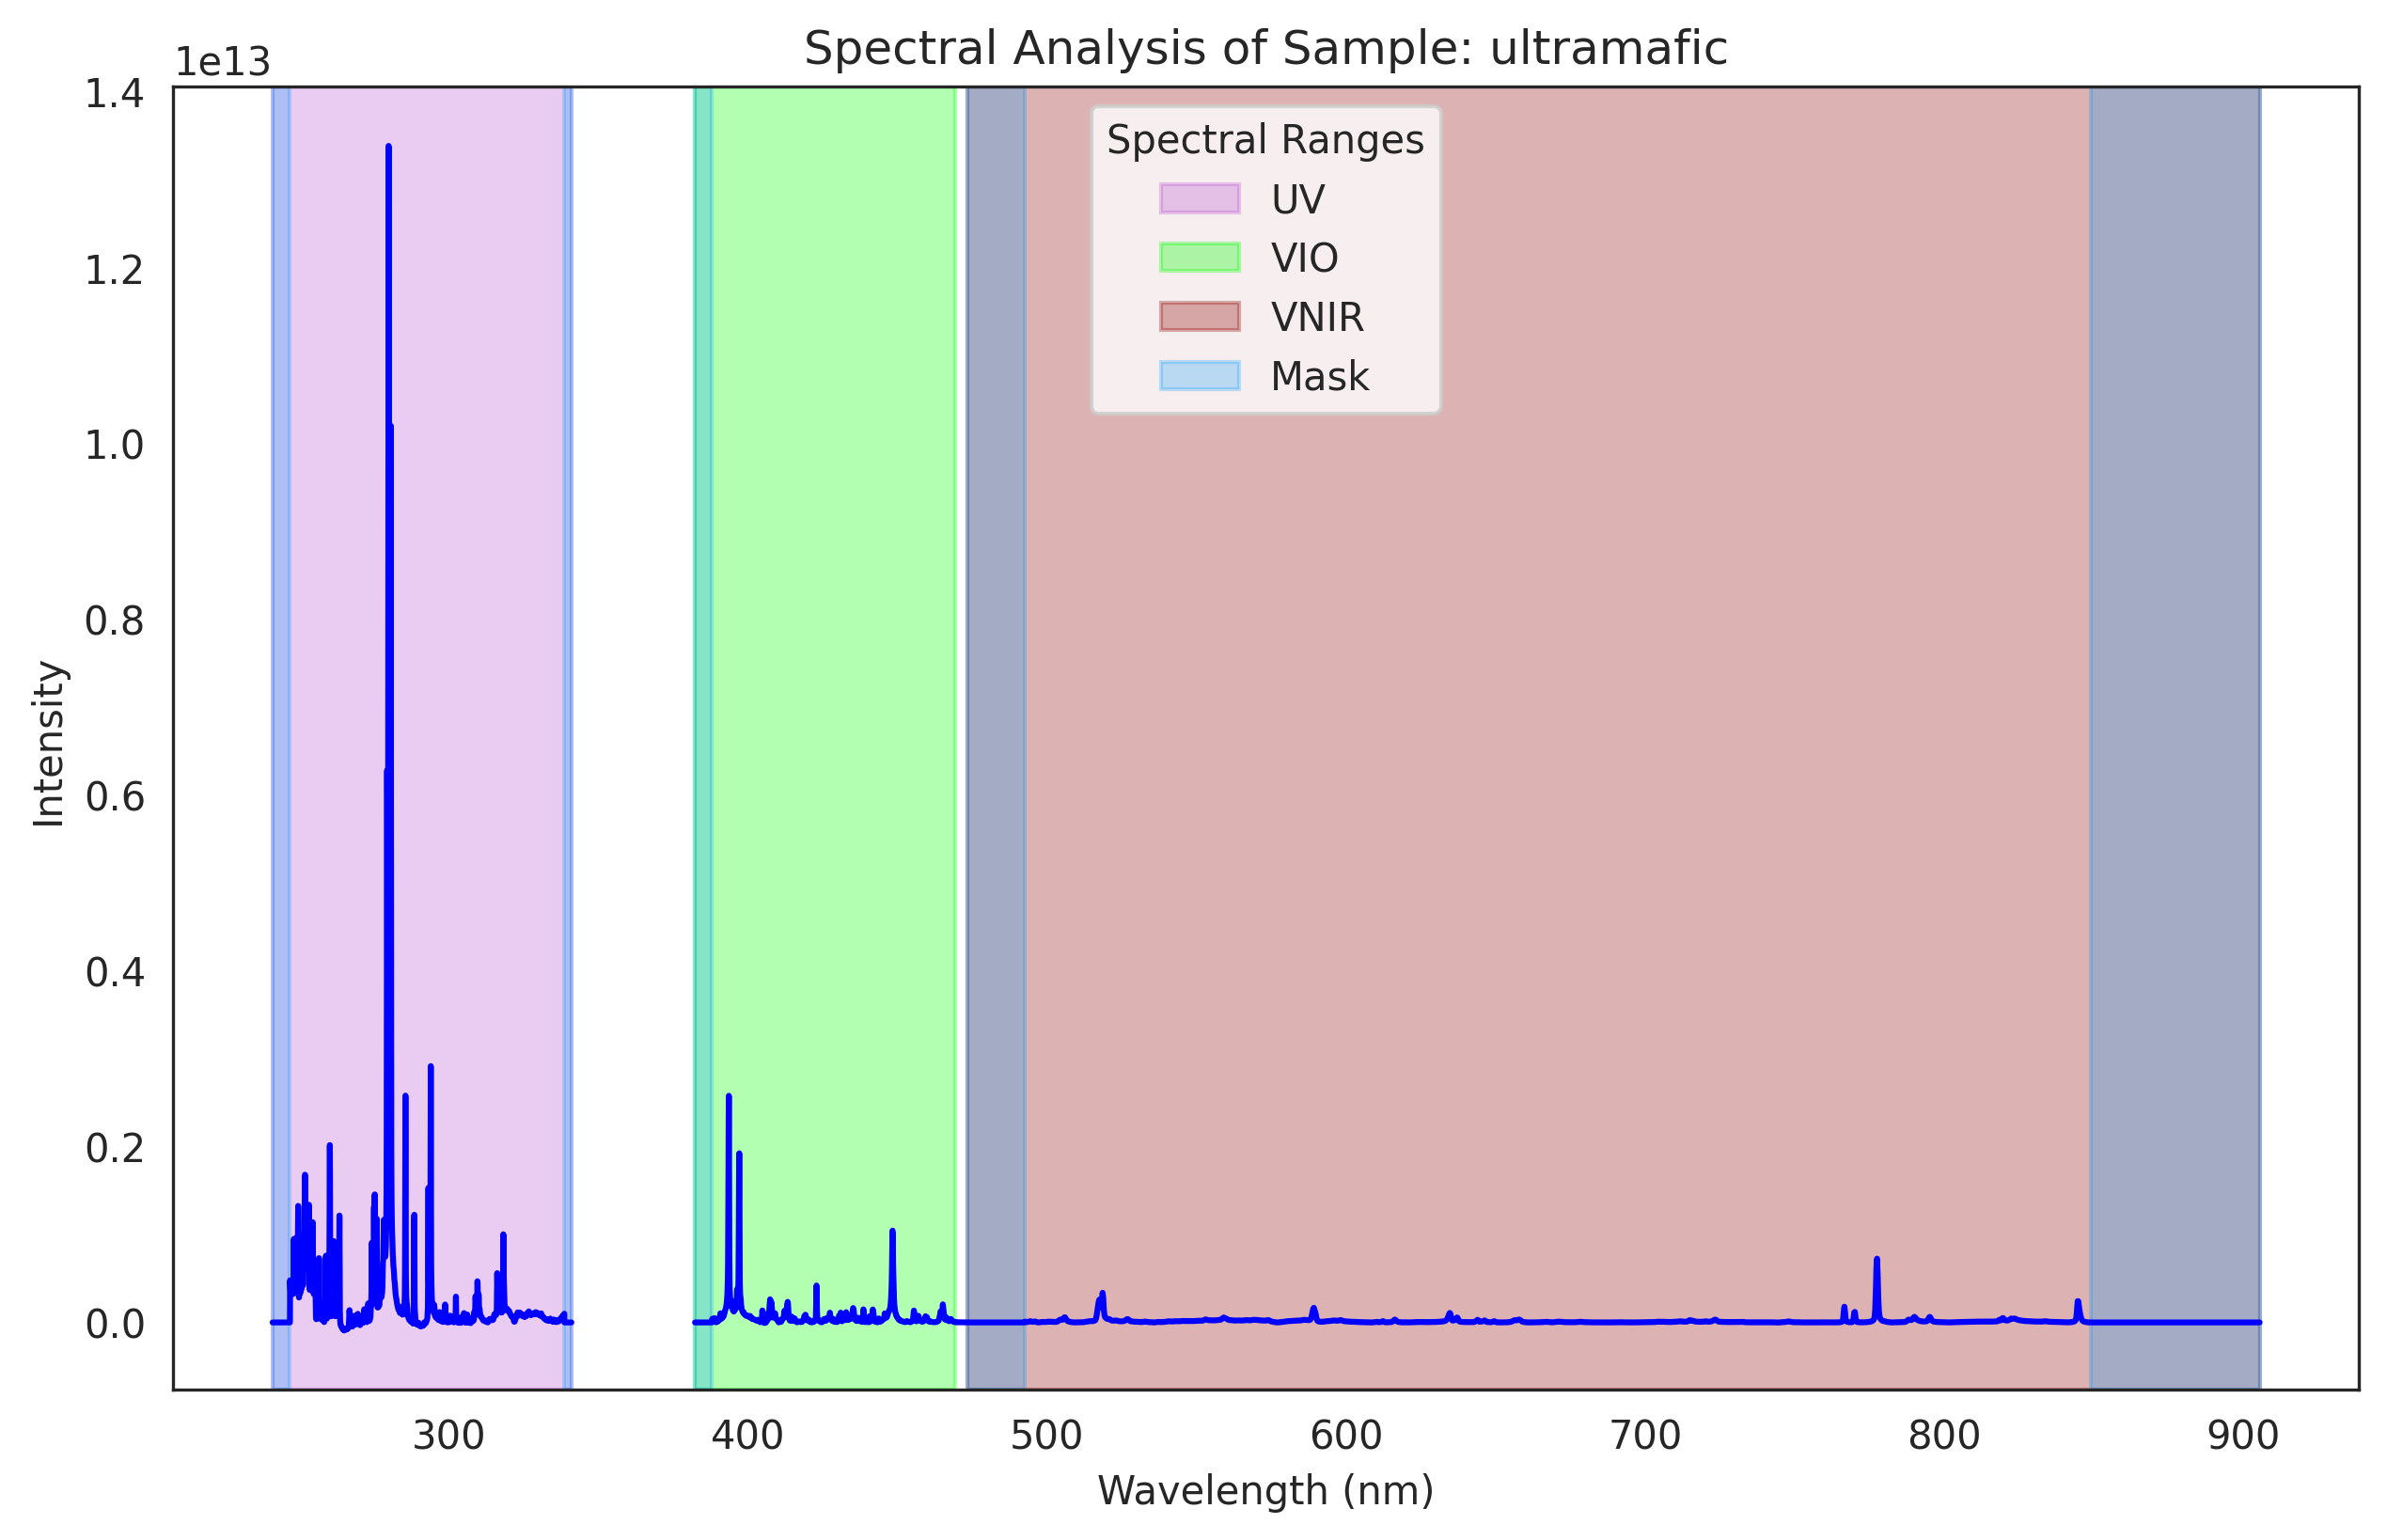
\includegraphics[width=0.5\textwidth]{images/spectral_plot.png}
	\caption{Spectral plot of the \gls{ccs} data for the \textit{ultramafic} sample. The wavelengths represent the spectral channels.}
	\label{fig:spectral_plot}
\end{figure}

Norm 3 can be understood as follows: for each sample, we consider the data from each spectrometer separately. Within each spectrometer, we divide the intensity of each channel by the sum of all channel intensities for that spectrometer. This process is applied for all three spectrometers, resulting in normalized data that preserves the relative intensities within each spectrometer while allowing for comparisons across different samples.

Formally, Norm 3 is defined as

\begin{equation}
	\tilde{X}_{i,j}^{(\gamma)} = \frac{X_{i,j}^{(\gamma)}}{\sum_{j=1}^{N} X_{i,j}^{(\gamma)}},
\end{equation}

where

\begin{itemize}
	\item $\tilde{X}_{i,j}^{(\gamma)}$ is the normalized wavelength intensity for the $i$-th sample in the $j$-th channel on the $\gamma$-th spectrometer with $\gamma \in \{1, 2, 3\}$,
	\item $X_{i,j}^{(\gamma)}$ is the original wavelength intensity for the $i$-th sample in the $j$-th channel on the $\gamma$-th spectrometer,
	\item $N = 2048$ is the number of channels in each spectrometer, and
\end{itemize}

This normalization method results in a total of $3N = 6144$ normalized features for each sample, as each of the three spectrometers contributes 2048 channels.

\subsubsection{Power Transformation}

\subsubsection{Quantile Transformer}

\subsubsection{Principal Component Analysis (PCA)}\label{subsec:pca}
\gls{pca} is a dimensionality reduction technique that transforms a set of possibly correlated variables into a smaller set of uncorrelated variables called \textit{principal components}.
We give an overview of the \gls{pca} algorithm based on \citet{James2023AnIS}.

First, the data matrix $\mathbf{X}$ is centered by subtracting the mean of each variable to ensure that the data is centered at the origin:

$$
\mathbf{\bar{X}} = \mathbf{X} - \mathbf{\mu},
$$

where $\mathbf{\bar{X}}$ is the centered data matrix and $\mathbf{\mu}$ is the mean of each variable.

The covariance matrix of the centered data is then computed:

$$
\mathbf{C} = \frac{1}{n-1} \mathbf{\bar{X}}^T \mathbf{\bar{X}},
$$

where $n$ is the number of samples.

Then, the covariance matrix $C$ is decomposed into its eigenvectors $\mathbf{V}$ and eigenvalues $\mathbf{D}$:

$$
\mathbf{C} = \mathbf{V} \mathbf{D} \mathbf{V}^T,
$$

where matrix $\mathbf{V}$ contains the eigenvectors of $\mathbf{C}$ and represents the principal component loadings.
These loadings indicate the directions of maximum variance in $\mathbf{X}$.
The matrix $\mathbf{D}$ is diagonal and holds the eigenvalues, each of which quantifies the variance captured by its corresponding loading.

These components are the scores $\mathbf{T}$, calculated as follows:

$$
\mathbf{T} = \mathbf{\bar{X}} \mathbf{V}_n,
$$

where $\mathbf{V}_n$ includes only the top $n$ eigenvectors.
The scores $\mathbf{T}$ are the new, uncorrelated features that reduce the dimensionality of the original data, capturing the most significant patterns and trends.

Finally, the original data points are projected onto the space defined by the top $n$ principal components, which transforms $X$ into a lower-dimensional representation:

$$
\mathbf{X}_{\text{reduced}} = \mathbf{\bar{X}} \mathbf{V}_n,
$$

where $\mathbf{V}_n$ is the matrix that only contains the top $n$ eigenvectors.

\subsubsection{Kernel PCA}
We provide a description of the \gls{kernel-pca} algorithm based on \citet{learningwithkernels}.
\gls{kernel-pca} is an extension of the traditional \gls{pca} that is used to handle nonlinear relationships among data points.
The core idea behind \gls{kernel-pca} is to map the data into a higher-dimensional space using a kernel function, known as the \textit{kernel trick}. 
This mapping allows for the linear separation of data points in the higher-dimensional space, even when the data is not linearly separable in the original space.

The core element of \gls{kernel-pca} is to obtain the covariance matrix in the higher-dimensional space. 
Mathematically, this is given by:
$$
	\mathbf{C} = \frac{1}{m} \sum_{j=1}^{m} \Phi(\mathbf{x}_j) \Phi(\mathbf{x}_j)^\top
$$
where $m$ is the number of data points and $\Phi(\mathbf{x}_j)$ represents the mapping of the data point $\mathbf{x}_j$ into the higher-dimensional feature space. 
The term $\frac{1}{m}$ normalizes the sum, ensuring the covariance matrix represents the average pairwise relationships between data points.

However, in practice, computing the covariance matrix is typically not feasible for large datasets, as computing the mapping function $\Phi(\mathbf{x}_j$ for each data point is expensive and often impractical due to the high dimensionality of the feature space. 
Instead, Kernel PCA leverages the kernel trick, which allows us to compute the similarity between data points directly in the original space using a kernel function $k(\mathbf{x}_i, \mathbf{x}_j)$. 
This kernel function implicitly computes the dot product $\Phi(\mathbf{x}_i)^\top \Phi(\mathbf{x}_j)$ in the higher-dimensional feature space without explicitly performing the mapping. 
By constructing the kernel matrix \(\mathbf{K}\) using these pairwise similarities, Kernel PCA can perform eigenvalue decomposition to obtain the principal components in the feature space, in the same fashion as regular \gls{pca} described in Section~\ref{subsec:pca}.
However, the eigenvalue decomposition is performed on the kernel matrix $\mathbf{K}$ rather than the covariance matrix $\mathbf{C}$.

\subsection{Overview of Core Models}
In this section, we provide an overview and definitions of \gls{pls}, \gls{svr}, \gls{etr}, \gls{gbr}, and \gls{xgboost}.
These models form the basis of the final architecture of our proposed pipeline, detailed further in Section~\ref{sec:methodology}.

\subsubsection{Partial Least Squares (PLS)}
Having previously introduced \gls{pca}, we now describe \gls{pls} based on \citet{James2023AnIS}.
In order to understand \gls{pls}, it is helpful to first consider \gls{pcr}, as \gls{pls} is an extension of \gls{pcr} that aims to address some of its limitations.

\gls{pcr} extends \gls{pca} in the context of regression analysis.
First, \gls{pca} is applied to the dataset $\mathbf{X}$, transforming it into a set of uncorrelated variables, the principal components.
These components, represented by scores $\mathbf{T}$, are derived from the eigenvectors $\mathbf{V}_n$ with the highest variances.

In \gls{pcr}, the dataset $\mathbf{X}$ is decomposed using PCA as:

$$
\mathbf{X} = \mathbf{TV}^T + \mathbf{E},
$$

where $\mathbf{T}$ represents the scores, and $\mathbf{V}$ represents the loadings.
\gls{pcr} utilizes these scores $\mathbf{T}$ in a linear regression model to predict the target variable $\mathbf{y}$:

$$
\mathbf{y} = \mathbf{Tb} + \mathbf{e},
$$

where $\mathbf{b}$ are the regression coefficients correlating $\mathbf{T}$ to $\mathbf{y}$, and $\mathbf{e}$ is the vector of residuals, capturing the prediction errors.

However, one drawback of \gls{pcr} is that it does not consider the target in the decomposition of the features and therefore assumes that smaller components have a weaker correlation with the target than the larger ones.
This assumption does not always hold, which is what \gls{pls} aims to address.

\gls{pls} uses an iterative method to identify components that maximize the covariance between the features and the target.
These components, $Z$, are linear combinations of the original features, $X_j$, weighted by coefficients, $\phi_j$, which are specifically calculated to reflect this covariance.
The formula for each component is expressed as:

$$
    Z = \sum_{j=1}^{p} \phi_j X_j,
$$

where $Z$ represents the component, $X_j$ is the $j$-th feature, and $\phi_j$ is the weight for the $j$-th feature.
The weights, $\phi_j$, are determined by the formula:

$$
    \phi_j = \frac{\text{cov}(X_j, Y)}{\text{var}(X_j)}.
$$

To refine the model iteratively, PLS uses the residuals from the previous components to calculate the next component.
The $m$-th component, for example, is derived from the residuals of the previous $m-1$ components:

$$
    Z_m = \sum_{j=1}^{p} \phi_{jm} \hat{X}_{j, m-1}.
$$

The components are then used to predict the target variable by fitting a linear model via least squares regression.

\subsubsection{Support Vector Regression (SVR)}
\gls{svr} is a regression technique that extends the principles of \gls{svm} to regression problems.
We therefore provide an overview of \gls{svm}s based on \citet{James2023AnIS} before discussing \gls{svr}s.

\gls{svm} is a supervised learning algorithm used primarily for classification tasks.
A core concept in \gls{svm} is the \textit{hyperplane}.
Generally, a hyperplane is a subspace of one dimension less than its ambient space.
This means that in a two-dimensional space, a hyperplane is a line, while in a three-dimensional space, it is a plane, and so on.

\gls{svm} is built on the idea of finding the hyperplane that best separates the data points into different classes.
This hyperplane is chosen to maximize the margin, which is the distance between the hyperplane and the nearest data point from either class.
The instances right on or inside the margin are called \textit{support vectors}, which are used to 'support' the margin and decision boundary.

\gls{svr} extends the principles of \gls{svm} to regression problems.
We use our previous discussion of \gls{svm} to introduce \gls{svr} based on \citet{druckerSVR}.

\gls{svr} aims to fit a function that predicts continuous values rather than finding the hyperplane that best separates data points.
Instead of using a hyperplane to separate the data, \gls{svr} uses two parallel hyperplanes to define a margin within which the function should lie, often referred to as the $\epsilon$-\textit{tube}, where $\epsilon$ is a hyperparameter that defines the width of the tube.
The goal is to find a function $f(x)$ that lies within this tube and has the maximum number of data points within the tube.
$f(x)$ is typically defined as a linear function of the form:

$$
f(x) = \mathbf{w} \cdot \mathbf{x} + b,
$$

where:

\begin{itemize}
	\item $\mathbf{w}$ is the weight vector,
	\item $\mathbf{x}$ is the input vector, and
	\item $b$ is the bias term.
\end{itemize}

The two parallel hyperplanes at a distance $\epsilon$ from the hyperplane are defined as:

$$
\begin{aligned}
    \mathbf{w} \cdot \mathbf{x} + b &= f(\mathbf{x}) + \epsilon, \\
    \mathbf{w} \cdot \mathbf{x} + b &= f(\mathbf{x}) - \epsilon.
\end{aligned}
$$

Or, more succinctly:

$$
\begin{aligned}
    f^+(\mathbf{x}) &= f(\mathbf{x}) + \epsilon, \\
    f^-(\mathbf{x}) &= f(\mathbf{x}) - \epsilon,
\end{aligned}
$$

where $f^+(\mathbf{x})$ and $f^-(\mathbf{x})$ are the upper and lower bounds of the $\epsilon$-insensitive tube, respectively.

The optimization problem in \gls{svr} is to find the coefficients $\mathbf{w}$ and $b$ that minimize the norm of $\mathbf{w}$ (i.e., keep the regression function as flat as possible) while ensuring that most data points lie within the $\epsilon$ margin.

\subsubsection{Extra Trees Regressor (ETR)}

\subsubsection{Gradient Boosting Regressor (GBR)}

\subsubsection{XGBoost}

\subsection{Stacking Ensemble}
% \citet{pavlyshenko2018stacking}

\section{Related Work}
In addressing the challenge of predicting major oxide compositions from \gls{libs} data, our investigation intersects with a broad spectrum of existing research that tackles similar computational hurdles, such as high dimensionality, multicollinearity, matrix effects, and the challenges of small datasets.
This section outlines how prior works relate to our problem, drawing from a range of techniques and methodologies that offer potential pathways for enhancing the accuracy and robustness of our predictions.

\citet{andersonPostlandingMajorElement2022} experimented with different machine learning models for quantifying major oxides on Mars using the SuperCam instrument on the Mars 2020 Perseverance rover.
They discuss preprocessing, normalization of \gls{libs} spectra, and the development of multivariate regression models to predict major element compositions.
For each oxide, they tested different models and selected the best performing one.
In some cases, they used a blend of models to improve the predictions.
The models they tested include: \gls{ols}, \gls{pls}, \gls{lasso}, Ridge, \gls{enet}, \gls{omp}, \gls{svr}, \gls{rf}, \gls{gbr}, and local \gls{enet} and blended submodels.
For \ce{SiO2}, they used a blend of \gls{gbr} and \gls{pls} models.
Interestingly, they found that PLS performed better at longer distances (4.25m), but GBR was better at 3m.
For \ce{TiO2}, they selected the \gls{rf} model for its superior performance at 4.25m and overall lower \gls{rmsep}.
For \ce{Al2O3}, they used an average of predictions from four models (Local \gls{enet}, \gls{rf}, two variants of \gls{pls}) to obtain the lowest \gls{rmsep}.
For \ce{FeO_T}, they initially selected \gls{rf} but later replaced it with \gls{gbr} due to its more realistic stoichiometry predictions for high-\ce{Ca} pyroxenes and overall performance.
For \ce{MgO}, they selected \gls{gbr} for having the lowest \gls{rmsep} and avoiding negative predictions, despite slightly overpredicting \ce{MgO} for high concentration samples.
For \ce{CaO}, they used a blend of \gls{rf} and \gls{pls} to address the bimodal distribution of \ce{CaO} predictions by the \gls{rf} model alone.
For \ce{Na2O}, they used a blend of \gls{gbr} and \gls{lasso} models to utilize \gls{gbr}'s accuracy at low concentrations and \gls{lasso}'s superior predictions at higher concentrations.
For \ce{K2O}, they selected \gls{lasso} for its better performance on high \ce{K2O} samples, despite the averaged model of five algorithms showing slight improvements at lower concentrations.
The findings of this paper are significant to us because they provide a benchmark for the performance of different machine learning models on \gls{libs} spectra.
We can use this information to guide our model selection and to compare our results with theirs.
Additionally, we might want to try out different models from the ones they tested to see if we can improve the predictions further, or perhaps find a model that is more suitable for our specific use case.
Also, SuperCam being the successor to \gls{chemcam} means that the findings of this paper are directly relevant to our work.

\citet{song_DF-K-ELM} present a novel approach to enhance the performance and interpretability of machine learning models in the context of \gls{libs} quantification.
The authors use "knowledge-based spectral lines, related to analyte compositions, to construct a linear physical principle based model and adopts \gls{k-elm} to account for the residuals of the linear model."
The method is based on \gls{df} and \gls{k-elm} and is called \gls{df}-\gls{k-elm}.
This method stands out by offering an intuitive explanation of how knowledge-based spectral lines impact prediction results, thereby enhancing model interpretability without compromising model complexity.
DF-\gls{k-elm} was tested across 10 regression tasks based on 3 \gls{libs} datasets, comparing its performance against six baseline methods using \gls{rmsep} as the evaluation metric.
They have 3 coal datasets, and they do regression tasks involving carbon, ash, volatile matter, and heat value analysis.
It achieved the best performance in 4 tasks and the second-best in 2 tasks, demonstrating its efficacy.
Incorporation of domain knowledge not only improved the accuracy of the models but also enhanced their generalizability across different tasks.
The method's design allows for a more interpretable machine learning model that adheres closer to the physical principles underlying \gls{libs} quantification.
The integration of domain knowledge into machine learning models addresses two critical challenges: improving the interpretability of complex models and enhancing their performance by leveraging specific domain insights.
The approach demonstrates a practical application of kernel extreme learning machines combined with domain-specific insights.
This is particularly valuable in fields like spectroscopy, where understanding the relationship between the spectral data and the analyte concentration is vital.
The DF-\gls{k-elm} method showcases how hybrid models can outperform traditional machine learning approaches.
The approach demonstrates a practical application of kernel extreme learning machines combined with domain-specific insights.
This is very relevant to our work considering interpretability is a key requirement for NASA and something they considered when choosing the \gls{pls} model for the \gls{chemcam} instrument.

\citet{rezaei_dimensionality_reduction} explore a variety of statistical and machine learning methods, including \gls{mulr}, \gls{svr}, \gls{ksvr}, and \gls{ann}, alongside their integrations with \gls{pca} to reduce dimensionality and improve model performance.
They use \gls{mse} and \gls{mae} as evaluation metrics to compare the performance of the models.
This paper clearly demonstrates the effectiveness of dimensionality reduction techniques in improving the performance of machine learning models because it compares the performance of many models with and without \gls{pca}: \gls{ann}, \gls{mulr}, \gls{svr}, \gls{ksvr}, \gls{pca}-\gls{ann}, \gls{pca}-\gls{mulr}, \gls{pca}-\gls{svr}, and \gls{pca}-\gls{ksvr}.
For all elements, a variant of \gls{svr} performs the best.
For \ce{Si}, \gls{svr} performs the best.
For \ce{Zn}, \gls{pca}-\gls{svr} performs the best.
For the rest of the elements, \gls{pca}-\gls{ksvr} performs the best.
The superiority of \gls{ksvr} is attributed to the its ability to handle non-linear relationships in the data effectively, especially when combined with \gls{pca}'s capability to compress and simplify the input data by focusing on the most relevant variations.

\citet{yang_laser-induced_2022} present a study on the application of a deep \gls{cnn} for classifying geochemical samples using \gls{libs}, with a particular focus on planetary exploration missions such as China's Tianwen-1 Mars mission.
The authors demonstrate the effectiveness of a deep CNN in classifying geochemical standard samples using \gls{libs} spectra collected at varying distances.
This addresses the challenge of spectral differences induced by distance, showcasing that \gls{cnn} can learn to classify samples without the need for traditional spectral preprocessing or distance correction.
Using a dataset of over 18,000 \gls{libs} spectra from 39 geochemical standard samples, the study compares the \gls{cnn} model's performance against four other machine learning models: \gls{bpnn} \gls{svm}, \gls{lda}, and \gls{logreg}.
The \gls{cnn} model exhibits superior classification accuracy, emphasizing its potential for geochemical sample identification/classification in planetary exploration.
The paper includes a detailed comparative analysis, proving the \gls{cnn} model's superior performance.
With classification accuracies on the validation set for all models exceeding 95\%, the \gls{cnn} model demonstrated the highest overall accuracy.
This was particularly evident as the training set size increased, indicating the model's robustness to varying distances without requiring distance correction.
Statistical analysis further confirmed the \gls{cnn} model's superiority, with higher average Ncorr values compared to other models.
The \gls{cnn} model's ability to accurately classify geochemical samples without preprocessing for distance correction is quite impressive.
This is particularly relevant to our work because we are also working with \gls{libs} spectra collected at varying distances.
The comparative analysis underscores the \gls{cnn} model as a best-fit approach for \gls{libs} data analysis, potentially setting a new standard for future research and applications in the field.

\citet{jeonEffectsFeatureEngineering2024} investigated the effects of feature engineering on the robustness of \gls{libs} for steel classification.
They developed a remote \gls{libs} system to classify six steel types, using various feature-engineering and machine learning algorithms, including \gls{svm} and \gls{fcnn}, to handle different laser energies in test datasets.
They found that using intensity ratios as input data resulted in more robust classification models.
It was better than \gls{pca} and \gls{rf}-based wavelength selection.
The study highlights the importance of selecting appropriate feature engineering methods to improve model robustness, especially under varying measurement conditions.
This is relevant to our project as it demonstrates how feature engineering can enhance the performance and robustness of models for classifying materials based on \gls{libs} data, addressing challenges similar to those we face in predicting major oxide compositions.

The study by \citet{fontanaLaserInducedBreakdown2023}.
explores using \gls{libs} for whole-rock geochemical analysis, specifically for major elements like \ce{Al}, \ce{Ca}, \ce{Fe}, \ce{K}, \ce{Mg}, \ce{Na}, \ce{Si}, and \ce{Ti}.
They averaged \gls{libs} spot analyses over 1-mm spaced transects on drill core intervals, demonstrating strong correlations with lab-based geochemistry for elements like \ce{Si}, \ce{Al}, and \ce{Na}.
Different predictive models were used for each element, such as \gls{pls}, \gls{enet}, \gls{lasso}, and \gls{pcr}, showing varied \gls{rmsecv} values indicating the precision of these models.
This method's relevance to our work lies in its potential for rapid, in-situ geochemical analysis, offering a way to overcome challenges related to high dimensionality and non-linearity in \gls{libs} data.

The paper by \citet{sunMachineLearningTransfer2021} introduces transfer learning to \gls{libs} spectral data analysis for rock classification on Mars, significantly improving model performance.
Previously, models trained on laboratory standards (pellets) struggled with physical matrix effects when applied to natural rock spectra.
Transfer learning, leveraging knowledge from one domain to address related problems in another, was applied to overcome this challenge.
The method showed remarkable improvement in \gls{tas} classification accuracy for both polished and raw rock samples, with rates increasing from 25\% and 33.3\% to 83.3\% respectively using machine learning models to 83.3\% with the transfer learning model.
This demonstrates the effectiveness of transfer learning in addressing the physical matrix effect and enhancing model robustness for rock classification on Mars.

\citet{wangDeterminationElementalComposition2023} discusses an advanced methodology for analyzing stream sediments using remote \gls{libs} combined with a \gls{mdsbpnn} algorithm.
This approach yielded highly accurate quantitative analyses of both major and trace elements, with determination coefficients (R2) for major elements exceeding 0.9996 and for trace elements greater than 0.9837, and \gls{rmse} less than 0.73 (major elements).
The study emphasizes the potential of remote \gls{libs} technology, especially for identifying biominerals in geological samples, highlighting its significance for studying ancient planetary environments.

% We had this one last semester IIRC. Might be good to have again?
\citet{leporeQuantitativePredictionAccuracies2022a} provides an in-depth analysis of the effectiveness of using \gls{libs} for geochemical analysis, focusing on the optimization of calibration datasets through the creation of submodels.
It outlines the methodology for collecting and processing \gls{libs} spectra, the development of multivariate models for predicting geochemical compositions, and compares the predictive accuracies of different submodel strategies.
The study finds that while submodels can improve prediction accuracies under certain conditions, the overall effectiveness is contingent upon having a large and diverse calibration dataset.
The research suggests that the optimal use of \gls{libs} for geochemical analysis requires a balance between the specificity of submodels and the breadth of the calibration dataset to ensure accurate and reliable predictions.

\citet{kepesImprovingLaserinducedBreakdown2022} discusses enhancing \gls{libs} model accuracy using transfer learning between ChemCam and SuperCam instruments.
It proposes a method where ChemCam data transforms to approximate SuperCam spectra, improving \gls{cnn} regression models' performance.
Key methods include data augmentation and fine-tuning of \gls{cnn}s with pre-processed and normalized spectra.
This approach outperforms some existing models for specific oxides, demonstrating transfer learning's potential in \gls{libs} analyses for more accurate quantitative models.

\citet{ferreiraComprehensiveComparisonLinear2022} presents an extensive comparison of various algorithms for quantifying lithium in geological samples, with a focus on both linear and non-linear methods.
The study tested algorithms on spectra acquired from a commercial handheld device and a laboratory prototype, highlighting the challenges in quantifying lithium due to effects like saturation and matrix interference.
The results showed that non-linear methodologies, such as \gls{knn} regression, \gls{svr}, and \gls{ann} regression, generally outperformed linear methods by effectively managing saturation and matrix effects, which are common in geological samples.
This research provides valuable insights for future applications in geological sample analysis and could potentially be generalized for other elements in similar contexts.
The paper's findings are particularly relevant to our project as it demonstrates the effectiveness of non-linear machine learning techniques in handling complex, non-linear relationships in high-dimensional \gls{libs} data, aligning with our research objectives of improving major oxide composition predictions from \gls{libs} data.

The study by \citet{liuComparisonQuantitativeAnalysis2022} explores the use of \gls{marscode} \gls{libs} for quantitative analysis of olivine in a simulated Martian atmosphere, focusing on multivariate analysis methods to address challenges posed by \gls{libs} data, such as high dimensionality and multicollinearity.
The methods evaluated include \gls{ulr}, \gls{mvlr}, \gls{pcr}, \gls{plsr}, ridge regression, \gls{lasso}, \gls{enet}, and \gls{bpnn}.
The findings demonstrate the effectiveness of dimension reduction techniques, especially \gls{plsr}, and nonlinear analysis for improving quantitative analysis accuracy of olivine using \gls{libs} data.
This approach is particularly relevant to our work due to the focus on advanced statistical methods and machine learning algorithms for handling complex, high-dimensional \gls{libs} data, aligning with our objectives of improving accuracy and robustness in predicting major oxide compositions.

\cite{yangConvolutionalNeuralNetwork2022} is a study where a \gls{cnn} model is designed to identify twelve types of rocks using \gls{libs} data from the \gls{marscode} for the Tianwen-1 Mars exploration mission.
The classification performance of the \gls{cnn} is compared with \gls{logreg}, \gls{svm}, and \gls{lda}.
The \gls{cnn} model achieved the highest classification accuracy, demonstrating its efficiency in rock identification with \gls{libs} spectra collected in a simulated Martian environment.
This indicates that \gls{cnn}-supported \gls{libs} classification is a promising analytical technique for planetary exploration missions.

\citet{silvaRobustCalibrationModels2022} introduce clustered regression calibration algorithms for \gls{libs} to address quantification challenges in complex sample matrices or wide concentration ranges, focusing on lithium quantification in geology.
They employ unsupervised clustering to group similar samples before applying a tailored linear calibration model to each cluster.
This approach, tested on lithium in exploration drills, outperforms standard linear models, especially in lower concentration regions, and demonstrates good generalizability to unseen data from different rock veins.
The study highlights the potential of clustered regression methods in improving \gls{libs} quantification accuracy and robustness, particularly valuable in mining environments.
Uses Ridge regression, \gls{pls}, dimensionality reduction with \gls{umap} and then k-means clustering, followed by a local model for each cluster, univariate calibration curves.

\citet{woldPrincipalComponentAnalysis1987} provides an in-depth tutorial on \gls{pca}, a fundamental method in multivariate data analysis used for dimensionality reduction, outlier detection, and uncovering the underlying structure in data sets.
The paper covers the history and development of \gls{pca}, its mathematical foundations, applications across various fields, and detailed instructions for data pre-treatment and \gls{pca} implementation.
It emphasizes \gls{pca}'s utility in simplifying complex data sets, enhancing interpretability, and supporting data analysis through the extraction of principal components that capture the most variance in the data.
This work is particularly relevant to our project as it underscores the importance of \gls{pca} in handling high-dimensional data, which aligns with our objectives of improving the prediction accuracy and interpretability of major oxide compositions from \gls{libs} data by effectively managing multicollinearity and high dimensionality challenges.

\citet{bankAutoencoders2021} details various autoencoder architectures and their applications in machine learning, emphasizing their role in dimensionality reduction, feature learning, and generative models.
It explores regularized, denoising, and variational autoencoders, highlighting their advantages in compressing data into lower-dimensional spaces while retaining essential information for reconstruction.
Autoencoders could significantly enhance our ability to handle the high-dimensional nature of \gls{libs} data.
By compressing spectral data into more manageable representations without losing critical information, we can improve model performance, especially in predicting major oxide compositions, by focusing on the most relevant features extracted from the compressed data representation.
This aligns with our objectives of efficient dimensionality reduction and robust predictive modeling.

In their work \citet{caruana_no_1997}, presents a method called \textit{Multitask learning}, which is a method of learning machine models on several related datasets. 
The motivation for this approach stems from the assumption that utilizing multiple, albeit related, datasets can enhance the model's ability to discern patterns and shapes within the data.
\citet{caruana_no_1997} suggest that leveraging shared representations for model training can enable the model to identify underlying attributes in other data sets, even when this new data is small.
This is interesting to our report as one of the major challenges in analyzing LIBS calibration data for Mars is the scarcity of available data.
This scarcity makes it difficult to construct robust models capable of comprehensively understanding the underlying patterns and physical principles within the data.
Utilizing related LIBS data could help the models first learn the general outline, shape and patterns in the LIBS data, making it easier for it to grasp the deeper patterns in the Mars related data.




\section{Definition}\label{sec:definition}
This section introduces the LIBS dataset and the hypothesis function for predicting the composition of major oxides, establishing the foundation for model evaluation and optimization in our study.

\begin{definition}\label{def:dataset}
    Let $D$ be the LIBS data set, defined in the space $\Lambda \times \mathbb{R}^m$, where $\Lambda$ represents the set of possible wavelengths and $\mathbb{R}^m$ denotes the $m$-dimensional space of intensities.

    The dataset $D$ is given by $D = \{ (\lambda_1, \vec{I}_1), (\lambda_2, \vec{I}_2), \ldots, (\lambda_n, \vec{I}_n) \}$, where each element $(\lambda_i, \vec{I}_i) \in \Lambda \times \mathbb{R}^{m}$ comprises the wavelength $\lambda_i$ of the $i^{th}$ measurement point, measured in nanometers, and an $m$-dimensional intensity vector $\vec{I}_i = [I_{i1}, I_{i2}, \ldots, I_{im}]$.
    This vector captures the intensity values at $\lambda_i$ for each of the $m$ shots, measured in units of photons per channel.
\end{definition}

\begin{definition}\label{def:hypothesis_function}
    Given a set of major oxides $O$ where $k=|O|$, define a model $M$ that learns a hypothesis function $f: \Lambda \times \mathbb{R}^m \rightarrow \mathbb{R}^k$ to predict the composition of the $k$ major oxides in geological samples.
    The output of the hypothesis function is a vector $\mathbf{\hat{y}} = [\hat{y}_{1}, \hat{y}_{2}, \ldots, \hat{y}_{8}]$ where $\hat{y}_{i}$ is the predicted weight percentage of the major oxide $o_i \in O$.
\end{definition}
The sum of the predicted weight percentages is not necessarily equal to 100\%, but is not expected to surpass 100\%.
The samples may contain other elements that are not considered major oxides, which would account for the difference.
If the sum of the predicted weight percentages is greater than 100\%, the model is overestimating the weight percentages, and represents a physical impossibility.

There are various methods to evaluate the performance of a model.
We use the average RMSE of the predictions for each oxide $\mathbf{\hat{y}}$ and actual values $\mathbf{y}$, denoted $E$, as the error metric for the model:

\begin{equation}\label{eq:avg_rmse_metric}
    E(M) = \frac{1}{k} \sum_{i=1}^{k} \sqrt{\frac{1}{m} \sum_{j=1}^{m} (\hat{y}_{ij} - y_{ij})^2}
\end{equation}

Where \( \hat{y}_{ij} \) is the \( i^{th} \) component of the output vector \( \hat{y} \) for the \( j^{th} \) sample in the dataset \( D \), as produced by the hypothesis function \( f \) of model \( M \). Similarly, \( y_{ij} \) is the actual weight percentage of the \( i^{th} \) major oxide \( o_i \in O \) for the \( j^{th} \) sample.

Let $M_{MOC}$ be the baseline model recreated based on the original MOC model. $M_{MOC}$ is comprised of various components.
Our plan is to perform a series of experiments on $M_{MOC}$ by making changes to a select number of these components.
By doing so, we transform the original model $M_{MOC}$ into a new model $M$, which retains most of the original components and structure of $M_{MOC}$, with the exception of the modified components.
We will conduct several different experiments, each targeting different components of the model.
For every experiment, we will note which specific parts of the model were altered.
The goal is to measure how each experiment affects the model's performance by looking at the difference in errors before and after the changes.

This leads us to the following challenge:

\textbf{Problem}: Given a series of experiments and the resulting models, identify the components that contribute the most to the overall error $E(M)$. 

\subsection{Data Analysis}\label{subsec:data_analysis}
Description of the samples used and their relevance.
Explain how and why these samples were chosen.
\section{Methodology}\label{sec:methodology}
As part of our goal to evaluate the performance of each of the components in the pipeline, the first step was to create a replica of the original pipeline described by \citet{cleggRecalibrationMarsScience2017}
Since we did not have access to the original source code implementing the pipeline, we have replicated it at accurately as we could based on the available information.
We have had to make some assumptions due to insufficient information regarding some components, which we detail in this section.
In addition, some aspects of the pipeline rely on qualitative assessments made by the original authors --- something we cannot do because we are not domain experts.
Consequently, our pipeline is not identical to the original, but we have strived to make it as close as possible while favoring conservative choices and omitting implementations where information about the original pipeline was unclear.
This decision was driven by the aspiration to ensure that the baseline results remained minimally influenced by our methodological choices.

This section is dedicated to describing the methodology of our pipeline, how it differs from the original, and which design choices we have made and why.
Furthermore, we delve into the experiments we have conducted to evaluate the performance of our pipeline such that we can identify the components that contribute the most to the overall error.

Section \ref{sec:methodology_pls1}, we focus on the specifics of the PLS1-SM phase, detailing its associated data preprocessing procedures.
In Section \ref{sec:methodology_ica} then details the ICA phase, including its unique data preprocessing steps.
Lastly, Section \ref{sec:methodology_moc} presents a description of the MOC phase of the pipeline.

\subsection{PLS1-SM}\label{sec:methodology_pls1}
The PLS1-SM phase in our pipeline largely follows the same approach as described in \citet{andersonImprovedAccuracyQuantitative2017} with a few exceptions.
We detail our approach and the differences from the original pipeline in this section.

\subsubsection{Data Preprocessing}\label{sec:pls1_data_preprocessing}
The preprocessing of the data is illustrated in Figure~\ref{fig:pls_data_preprocessing}.

\begin{figure}
	\centering
	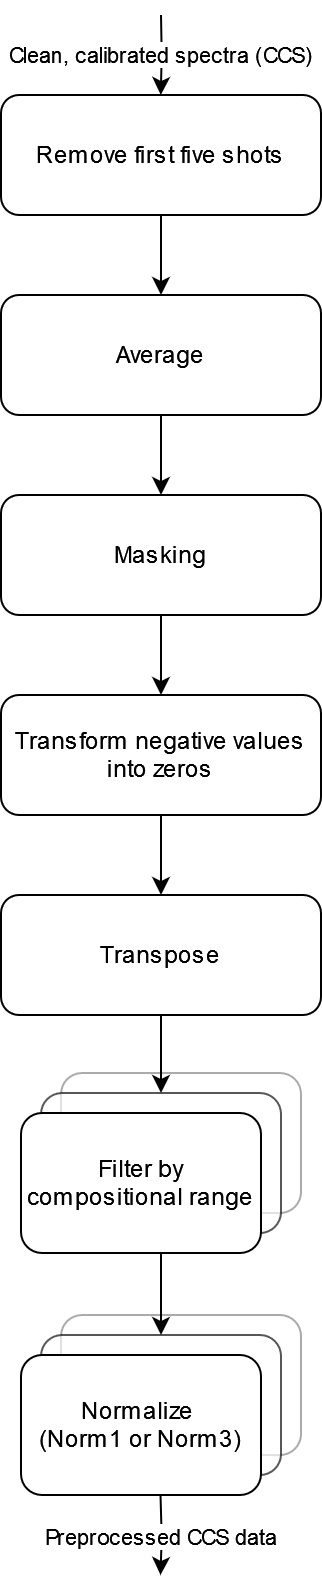
\includegraphics[width=0.175\textwidth]{images/pls_preprocessing.png}
	\caption{The PLS1-SM data preprocessing phase in our recreation of the pipeline. The filtering and normalization steps are done independently for each oxide.}
	\label{fig:pls_data_preprocessing}
\end{figure}
\noindent
We start by removing the first five shots from the data similarly to \citet{cleggRecalibrationMarsScience2017} since they are typically contaminated by dust that covers the target before being removed by the laser-produced shock waves.
Then the remaining 45 shots from each location are averaged, resulting in a single spectrum per location with a total of five spectra per target.
As mentioned in Section~\ref{sec:data_overview}, the edges of the spectral regions contain noise, so we apply masking to the data to remove these regions.
The masked regions, which do not contain unique major element diagnostic peaks, are excluded to enhance the accuracy and reliability of the quantitative analysis\cite{cleggRecalibrationMarsScience2017}.
The dataframe is then transformed through a transpose operation, swapping the rows and columns.
This gives us a dataframe with the average intensities per sample as rows, and the wavelengths as columns.
All negative values are then transformed into zeros since negative values are not physically possible.
Given the pre-defined compositional ranges for each oxide in \citet{andersonImprovedAccuracyQuantitative2017}, we filter out wavelengths outside of these ranges.
The range is defined by an upper and a lower bound, and any wavelength outside of this range is removed.
Finally, we apply two different normalization techniques, Norm1 and Norm3, to the data.
This results in two separate datasets, each normalized in a distinct manner but derived from the same original dataset.
ICA and PLS-SM are then performed on each of these datasets separately.
The reason for this is that, as \citet{cleggRecalibrationMarsScience2017} found, some of the oxides are better modeled with data normalized using Norm1, while others are better modeled with data normalized using Norm3.

\subsubsection{PLS1-SM Regression}\label{sec:methodology_pls1-sm_regression}
The PLS phase of the pipeline follows a submodel approach to make wt. \% predictions for each oxide, as previously mentioned in Section~\ref{sec:introduction}.

%TODO add information about the hyperparameters used
The training of the models follows the same approach as described in \citet{andersonImprovedAccuracyQuantitative2017} and is illustrated in Figure~\ref{fig:pls_training}.
However, assumptions have been made regarding the k-fold cross-validation process, as the authors are ambiguous in their description of the number of folds used.
We interpreted their description as using a 20\% holdout split and a 4-fold on the remaining 80\% of the data --- resulting in a total of 5 folds.
Furthermore, we have decided to automate outlier removal as described in Section~\ref{sec:methodology_outlier_removal} rather than performing it manually.
Finally, similar hyperparameters have been used for the PLS models as described in \citet{andersonImprovedAccuracyQuantitative2017}.

\begin{figure}
	\centering
	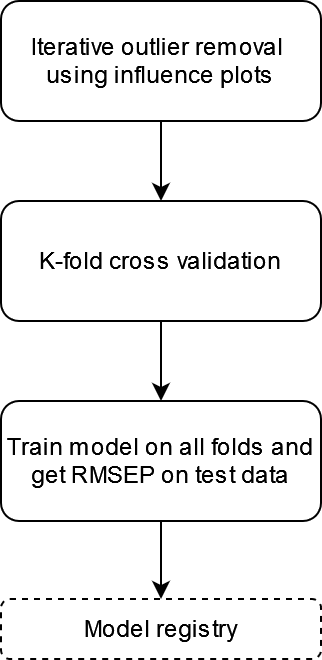
\includegraphics[width=0.175\textwidth]{images/pls_training.png}
	\caption{The PLS1-SM training phase in our recreation of the pipeline. This phase is repeated for each oxide's compositional range.}
	\label{fig:pls_training}
\end{figure}

Obtaining predictions for each of the eight oxides, for a single spectrum, requires a separate predictions for each oxide. While PLS regression is capable of multivariate regression, each oxide calls for different hyperparameter configurations and normalization procedures.
The submodels for an oxide generally include a full model, a low, mid, and high model. They are named after the compositional range in the data they are trained on. Here, compositional range refers to the known compositional values for a sample, which we use to filter the sample data to include samples data within that range.
These compositional ranges overlap, which creates a blending range.
Some oxides have only two compositional ranges, which means the model may have low-high as a blending range.

As mentioned, the PLS submodels approach is repeated for each oxide and is illustrated in Figure~\ref{fig:pls_inference}.
Given some new data sample, the full model gives an initial compositional prediction for its oxide.
Based on this prediction, the data is then "binned" into one of five concentration ranges -- the three submodel ranges and two blending ranges.
For each of these five concentration ranges, there is one or two corresponding \textit{submodel(s)}.
These submodels are used to make predictions in the corresponding concentration range after the full model has made its initial predictions.
The submodels are specialized in either low, low-mid, mid, mid-high, high concentration ranges, which are defined in Table 2 in \citet{andersonImprovedAccuracyQuantitative2017}.
If the full model predicts a concentration that falls within a blending range, the approach described in Section~\ref{sec:pls_submodels} is used to combine the predictions from the corresponding submodels.

\begin{figure}
	\centering
	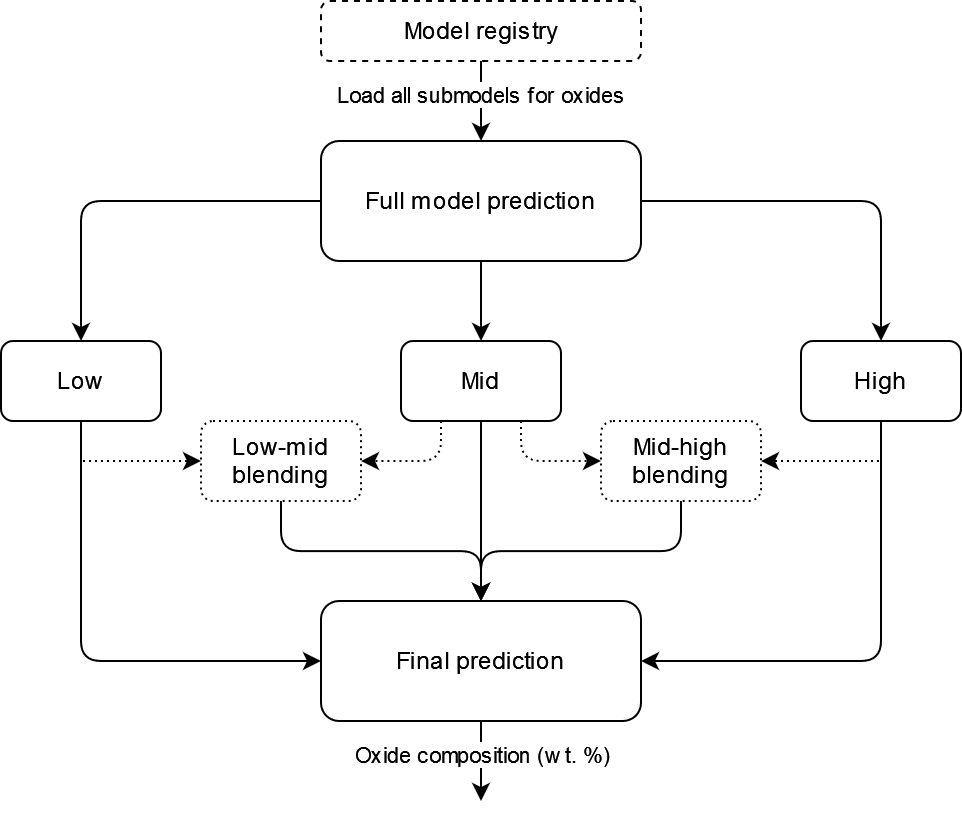
\includegraphics[width=0.45\textwidth]{images/pls_inference.png}
	\caption{The PLS1-SM inference phase in our recreation of the pipeline.}
	\label{fig:pls_inference}
\end{figure}

\subsubsection{Outlier Removal with Mahalanobis Distance and Chi-Squared Test}\label{sec:methodology_outlier_removal}
As mentioned in section \ref{sec:outlier_removal}, if the Mahalanobis distances can be shown to follow a chi-squared distribution, then the chi-squared test can be used to determine whether a sample is an outlier.
Since we do not have the expertise to make a qualitative assessment of the outliers, we have instead decided to use this property of the Mahalanobis distances to automatically detect outliers.
This works by computing the Mahalanobis distance for each data point in the training set, followed by a comparison of these distances against a chi-squared distribution.
A data point is classified as an outlier if its Mahalanobis distance corresponds to a chi-squared statistic that exceeds the critical value of the chi-squared distribution, which is determined by the specified degrees of freedom $\nu$.
The critical value is determined by the significance level $\alpha$ and $\nu$.
Since we have leverage and spectral residuals as our two dimensions, we have $\nu = 2$, because the number of dimensions is equal to the number of degrees of freedom\cite{aggarwal_outlier_2017}.

The outlier removal process is done iteratively because of the phenomenon described in \citet{cleggRecalibrationMarsScience2017} where removing outliers can cause new outliers to appear.
The process is as follows:
\begin{enumerate}
    \item Compute the Mahalanobis distances for each sample in the training set.
    \item Determine chi-squared statistics for these distances.
    \item Eliminate outliers exceeding the chi-squared critical value.
    \item Train a new model on the remaining samples.
    \item Repeat until model no longer improves as measured by the RMSE.
\end{enumerate}

It should be noted that our outlier removal process is conservative to avoid removing too many samples and as such, we have set our significance level $\alpha$ to 0.975.
This means that we are willing to accept a 2.5\% chance of falsely removing a sample that is not an outlier.

\subsection{ICA}\label{sec:methodology_ica}
The ICA phase in our pipeline can be seen in figure \ref{fig:ica_phase}.
In this section, we delve into the differences between our pipeline and the original, and we discuss the rationale behind our choices.

\begin{figure}
	\centering
	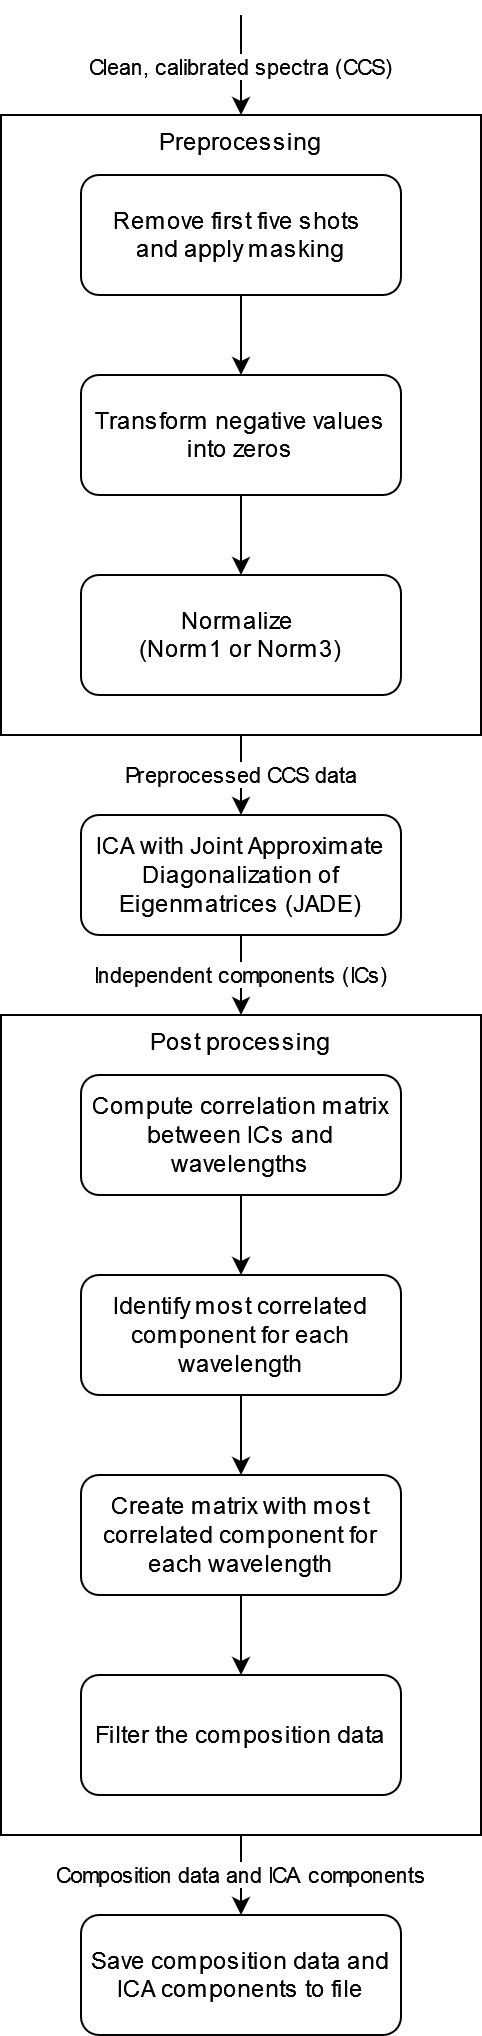
\includegraphics[width=0.2675\textwidth]{images/ica_phase.png}
	\caption{The ICA phase in our recreation of the pipeline.}
	\label{fig:ica_phase}
\end{figure}

\subsubsection{Data Preprocessing}\label{sec:ica_data_preprocessing}
For ICA, the first five shots are removed from the data.
We then apply masking to the data to remove the same regions as in the PLS1-SM phase.
Afterwards, we transform all negative values into zeros.
Then we normalize the data using Norm1 and Norm3.

In contrast to \citet{cleggRecalibrationMarsScience2017} however, we do not weigh by the inverse of the instrument response function (IRF) before normalizing.
The purpose of the IRF is to calibrate the measured signal to physical units since different pixels have different sensitivities\cite{wiensChemcam2012}.
One argument for inverting the IRF is that it introduces more noise in areas of interest on the spectrum by multiplying with a high value as part of the conversion to physical units.
However, during a conversation with one of the original authors of \citet{cleggRecalibrationMarsScience2017}, criticism was raised against this.
Specifically, the author pointed out that weighing by the inverse of the discards the alignment between the spectral data collected by the instrument in Los Alamos and the spectral data collected by the instrument on Mars.
If the same instrument were used for all analyses, one could argue that the IRF (apart from the inverse square law correction) part is irrelevant, but that is not the case here; there are two different instruments --- one in Los Alamos and one on Mars.
Based on these considerations, we have decided to not weigh by the inverse of the IRF.

In addition, because \citet{cleggRecalibrationMarsScience2017} does not mention how each of the five location datasets are used for each sample, we have decided to only use one for each sample.
This likely does not produce as accurate results as using all five location datasets would, since we do not get a full representation of the sample that was shot at by the laser, instead only getting a partial representation from a single location.
Nevertheless, to avoid deviating significantly from \citet{cleggRecalibrationMarsScience2017}'s methodology or making unfounded assumptions about their data processing, we have opted for this more conservative approach.
Our goal is to test each of the components of the pipeline individually rather than trying to reproduce the results to absolute perfection.

Similarly, in our replica of the pipeline, we have not incorporated outlier detection in the ICA part of the pipeline primarily because \citet{cleggRecalibrationMarsScience2017} does not describe their implementation sufficiently enough for replication without unsubstantiated assumptions.
They mention the use of Median Absolute Deviation for this purpose, but the specifics of their approach remain unclear.
Our decision to omit outlier detection in the ICA phase of our pipeline is also influenced by a preference for retaining a more comprehensive dataset, despite the potential inclusion of outliers.
Further supporting this decision is input from one of the original authors involved in the ChemCam project.
This author highlighted the extensive efforts invested in developing the ChemCam calibration dataset, suggesting a low presence of significant outliers.
While it would be ideal to include outlier detection in the ICA phase to ensure alignment with the original pipeline, implementing it based on substantial assumptions would be counterproductive, potentially compromising the integrity of our analysis.

After examining the results in section \ref{sec:results}, we will discuss the implications of these design choices in section \ref{sec:discussion}.

\subsubsection{Joint Approximate Diagonalization of Eigenmatrices (JADE) and Regression}
After preprocessing the data, we are ready to perform ICA.
This is done using the Joint Approximate Diagonalization of Eigenmatrices (JADE) algorithm, which is used to calculate the mixing matrix.
This mixing matrix is an $N \times M$ matrix, where $N$ is the number of samples and $M$ is the number of independent components.
By taking the product of the mixing matrix and the normalized data, we get the estimated sources.
This new matrix is an $M \times P$ matrix, where $M$ is the number of independent components, and $P$ is the number of wavelengths.

After performing ICA, we post-process by computing the correlation between the independent components and the wavelengths.
Using this, we can identify which wavelengths are associated with which independent components by computing the maximum correlation for each wavelength.
This gives us a matrix of ICA scores that we then use for regression.

\begin{figure}
	\centering
	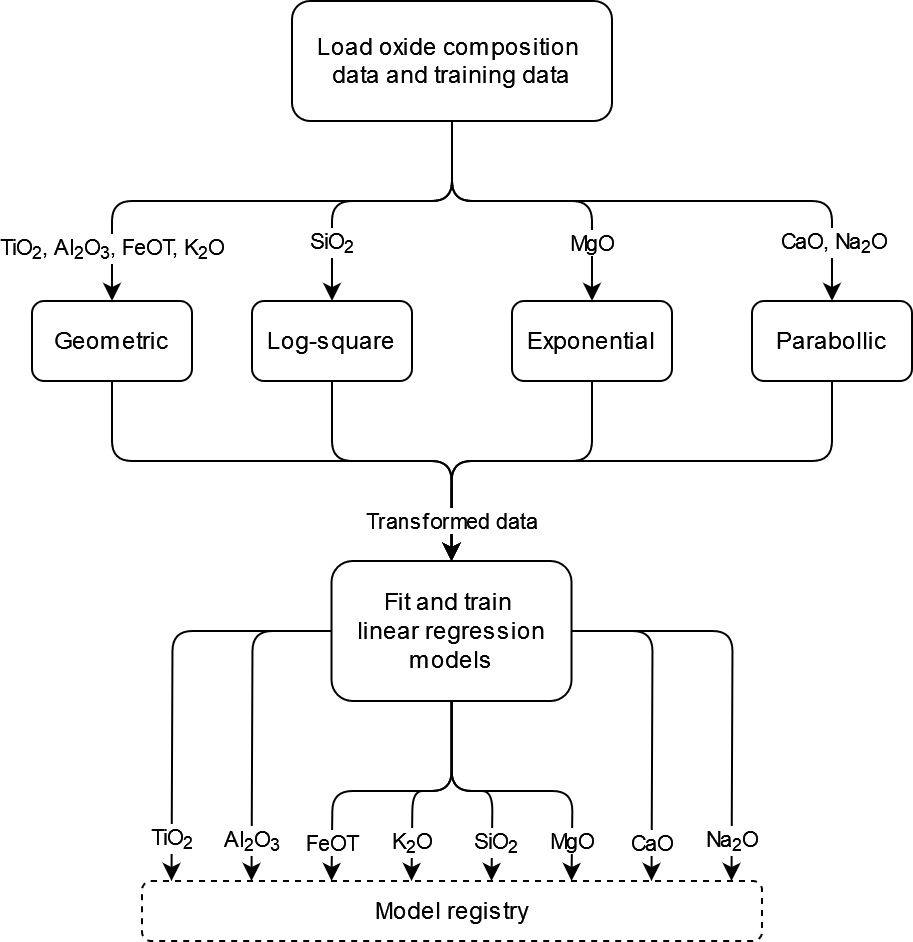
\includegraphics[width=0.45\textwidth]{images/ica_regression.png}
	\caption{Regression in the ICA phase of our recreation of the pipeline.}
	\label{fig:ica_regression}
\end{figure}

The regression process is illustrated in figure \ref{fig:ica_regression}.
\citet{cleggRecalibrationMarsScience2017} perform four more types of regression in addition to linear regression, namely parabolic, exponential, geometric and logsquare.
For each oxide, they used the type of regression and normalization that produced the best results.

We use Linear Regression for all oxides and instead transform the data to fit the model similar to \citet{kuo_detecting_2018}.
Initially, it might appear limiting, but by applying transformations to the features --— for example by taking logs, square roots, etc. --- it's possible to achieve an almost linear relationship with the target variable.

% TODO: Move this table to the results section and embed our own results in it as well to show the baseline results compared to the original results.
% This can be seen in table \ref{tab:regression_types}, which is taken from \citet{cleggRecalibrationMarsScience2017}.

% \begin{table}[h]
% \centering
% \begin{tabular*}{\columnwidth}{@{\extracolsep{\fill}}lccc}
% \toprule

% Element & Norm & Law type    & RMS \\ \midrule
% Si      & 1    & Logsqaure   & 6.7 \\
% Ti      & 3    & Geometric   & 0.6 \\
% Al      & 3    & Geometric   & 4.4 \\
% Fe      & 1    & Geometric   & 2.2 \\
% Mg      & 1    & Exponential & 3.0 \\
% Ca      & 1    & Parabolic   & 1.0 \\
% Na      & 3    & Parabolic   & 0.6 \\
% K       & 3    & Geometric   & 0.4 \\
% \bottomrule
% \end{tabular*}
% \caption{The summary of each ICA model characteristics from \citet{cleggRecalibrationMarsScience2017}.}
% \label{tab:regression_types}
% \end{table}

\subsection{MOC}\label{sec:methodology_moc}
As described in section \ref{sec:moc_derivation}, the result of the PLS1-SM and ICA are combined to produce the final MOC model, which weights the results of the two techniques in favor of the one that performs best for each oxide.
The specific weights used for each oxide can be seen in table \ref{tab:weighted_sum_oxide}.
Note that the weights for Ti, Mg and Ca have been set to 50/50 since \citet{cleggRecalibrationMarsScience2017} does not mention the weights they used for these elements.

\begin{table}[h]
\centering
\begin{tabular*}{\columnwidth}{@{\extracolsep{\fill}}lcc}
\toprule
Element  & PLS1-SM (\%) & ICA (\%) \\ \midrule
Al       & 75           & 25      \\
Fe       & 75           & 25      \\
Si       & 50           & 50      \\
Na       & 40           & 60      \\
K2       & 25           & 75      \\
Ti*      & 50           & 50      \\
Mg*      & 50           & 50      \\
Ca*      & 50           & 50      \\
\bottomrule
\end{tabular*}
\caption{Weighted Sum of Oxide Percentages. Elements marked with an asterisk (*) have been set to 50/50 as they are unspecified in \citet{cleggRecalibrationMarsScience2017}}
\label{tab:weighted_sum_oxide}
\end{table}

\subsection{Experiments}\label{sec:methodology_experiments}
To evaluate the performance of each of the components in the pipeline, we focus our experiments on three main aspects:

\begin{itemize}
	\item \textbf{Outlier removal} to assess the impact of leaving outliers in the dataset or using a different outlier removal method.
	\item \textbf{Hyperparameter tuning} to assess the impact of different hyperparameter configurations.
	\item \textbf{Other models} to compare the performance of the PLS1-SM and ICA models to other models.
\end{itemize}

\noindent
Given that the original authors did not perform experiments using alternative methods to demonstrate the efficacy of their chosen approach, this omission results in a lack of comprehensive understanding regarding the full potential of the pipeline's performance.
While they did perform hyperparameter tuning, they did not conduct experiments using different outlier removal methods or alternative models.
This raises questions about the optimality of the chosen methodology, as a comparative analysis with different methodologies could reveal superior approaches.
Experimenting with alternative methods means that we can uncover which components contribute the most to the overall error and therefore would benefit the most from further research and development.
Should a substitution of a component within the pipeline with an alternative method yield improved outcomes, it would indicate that the currently employed method represents a limitation in the overall pipeline, thus highlighting an area that necessitates enhancement.

\subsubsection{Experiment: Outlier Removal}\label{sec:experiment_outlier_removal}
The original PLS1-SM identified outliers manually by inspecting the leverage and spectral residuals plots.
We have instead chosen to automate this based on the reasons described in Section~\ref{sec:methodology_outlier_removal}.
It would therefore be intriguing to examine the impact on the pipeline's performance when this process is adjusted.
Firstly, examining the performance implications of completely omitting outlier removal would be worthwhile.
This experiment is justified given the substantial efforts dedicated to developing the ChemCam calibration dataset as mentioned in Section~\ref{sec:ica_data_preprocessing}, which implies a minimal presence of significant outliers.
Furthermore, experimenting with various significance levels for the chi-squared test could reveal whether a more or less conservative approach is advantageous.

In the ICA phase, the original authors employed the Median Absolute Deviation (MAD) for outlier removal, yet the detailed methodology of their approach was not fully delineated.
Consequently, in our version of the pipeline, we chose to exclude the outlier removal step during the ICA phase to avoid introducing unsubstantiated assumptions, as described in Section~\ref{sec:ica_data_preprocessing}.
This decision allows us to evaluate the intrinsic effectiveness of the ICA phase without the influence of outlier removal.
Introducing outlier removal using MAD in our replication of the pipeline presents an opportunity to assess its impact on the pipeline's efficacy.
By comparing the results with and without MAD, we can quantitatively measure the utility of this step.
Such an experiment is crucial for understanding whether MAD significantly contributes to reducing noise and improving data quality, thereby enhancing the overall performance of the machine learning pipeline.
This experiment would also offer insights into the robustness of the ICA phase against outliers, providing a more comprehensive understanding of the pipeline's capabilities and limitations.

\subsubsection{Experiment: Hyperparameter Tuning}\label{sec:experiment_hyperparameter_tuning}
\citet{cleggRecalibrationMarsScience2017} use qualitative judgement to identify hyperparameters for their PLS1-SM model.
This approach carries a risk of inaccuracies without sufficient domain expertise, given the challenges in guaranteeing the optimality of chosen hyperparameters.
Lacking such expertise, we opted for a more systematic and automated methodology to determine hyperparameters for our PLS1-SM model.

Similarly, the authors use eight independent components for their ICA algorithm, but do not provide any experimental results justifying that this is the optimal number of components.
As such, it is possible that the performance of the ICA phase could be improved by experimenting with a variety of components.

For the PLS1-SM model we decided to use the common grid search algorithm for testing different hyperparameters for the PLS models.
% Explain set up...

Since each independent component does not necessarily correlate one-to-one with the number of elements that one wishes to identify in a spectra, we decided to experiment with a number of components ranging between 4 and 25.
This range is within the vicinity of the original selection of components whilst providing us with a set of reasonable extremes.

% Probably show the setup in some way

\subsubsection{Experiment: Other Models}\label{sec:experiment_other_models}
\citet{cleggRecalibrationMarsScience2017} have only compared their new approach with the original method presented by \citet{wiensPreFlight3}, and have not conducted experiments using alternative methods to establish the superiority of their chosen approach.
Therefore, we decided to compare the performance of the PLS1-SM and ICA models to other models.
The objective is to evaluate two distinct scenarios. In the first scenario, we aim to conduct a direct comparison between the MOC model and an alternative model. The second scenario revolves around substituting either PLS or ICA with a different model and then calculating a weighted average.
We have decided to conduct the experiments using the following models:

\begin{itemize}
	\item \textbf{XGBoost}, a gradient boosting algorithm, \cite{chen_xgboost_2016}.
	\item \textbf{ANN}, a neural network model, \cite{scikit-learn}.
	% More? Random Forest, SVM, etc.
\end{itemize}

\section{Results}
We present the results of our experiments in this section.

\subsection{Visual and Statistical Analysis of \ce{SiO_2} Distribution in Partitioned Data}\label{sec:visual_analysis}
This section provides a detailed visualization and statistical analysis of the \ce{SiO_2} concentration distribution across data partitions, following the customized k-fold data partitioning procedure described in Section~\ref{subsec:validation_testing_procedures}.
We perform this analysis to validate the consistency of our data partitioning method and to provide a visual understanding of the data distribution it creates.
The analysis focuses on \ce{SiO_2} as a representative example.
We have conducted similar analyses for other oxides, but they are omitted here for brevity.

Figures \ref{fig:histogram_grid_plot} and \ref{fig:histogram_kde_plot} illustrate the histograms and \gls{kde} curves for \ce{SiO_2} concentrations in each training fold, the test set, and their combined distributions.
The consistent histograms and \gls{kde} curves across different training folds indicate that the data distribution within each fold closely matches the overall distribution, confirming their consistency and representativeness.

Figure \ref{fig:original_and_post_fold_plot} contrasts the \ce{SiO_2} concentration distribution before and after data partitioning.
The left plot shows the original distribution, while the right plot displays the fold-assigned distribution, color-coded by fold.
This visualization highlights that the partitioning strategy maintains the overall data distribution while ensuring balanced representation across folds.

\begin{figure*}[h!]
    \centering
    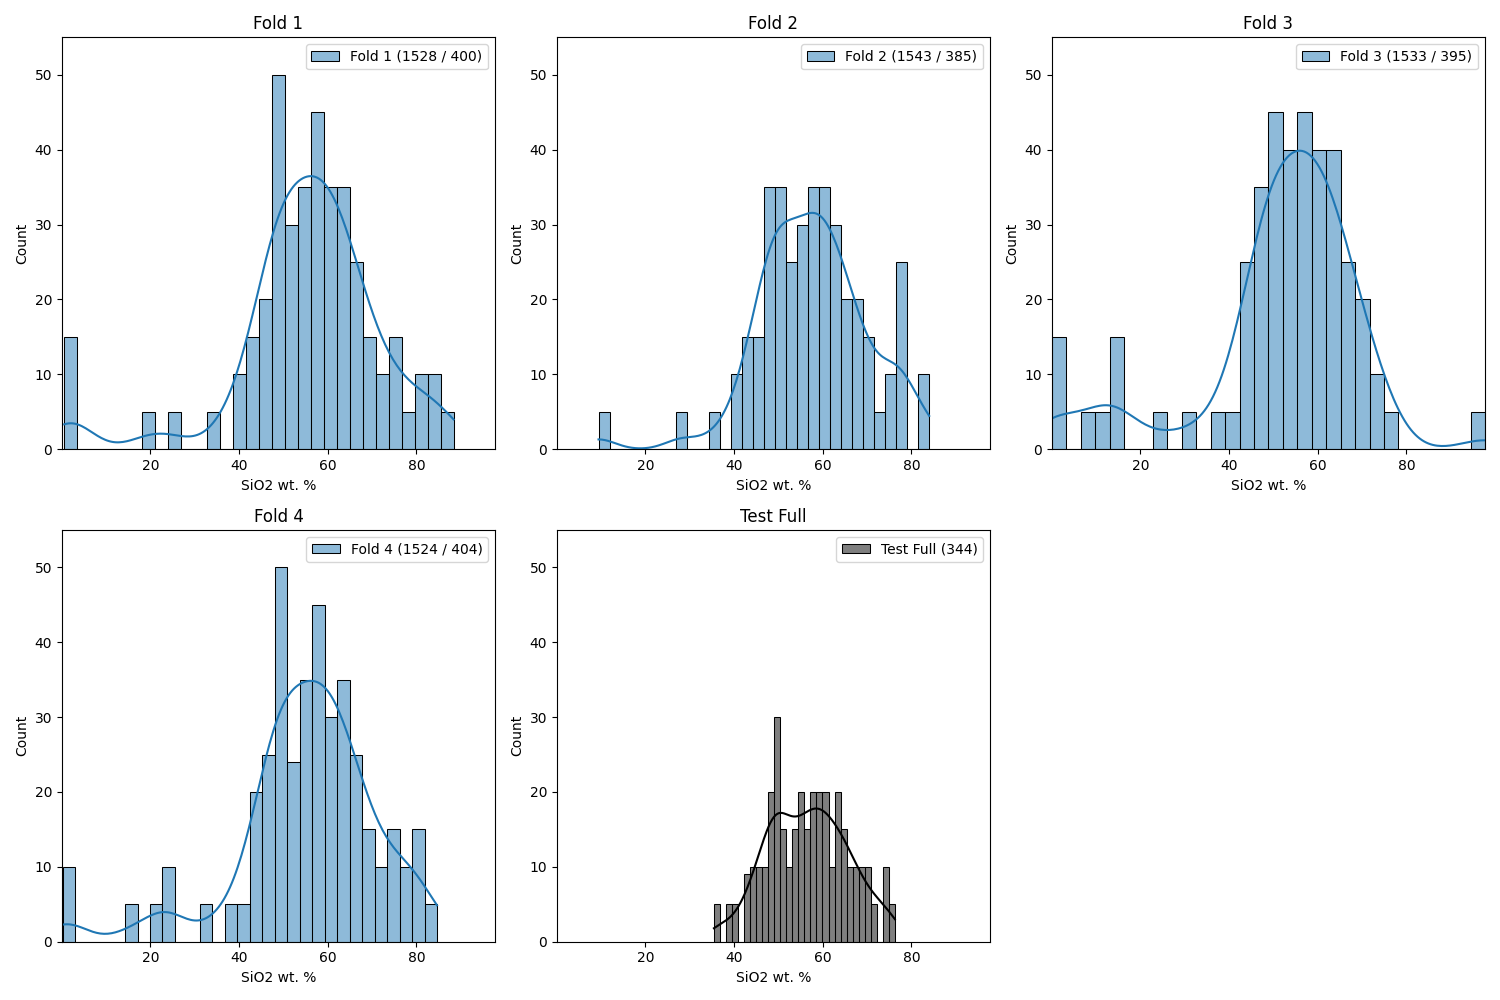
\includegraphics[width=\textwidth]{images/histogram_grid_plot.png}
    \caption{Histogram and \gls{kde} of \ce{SiO_2} Distribution in Each Fold. The y-axis represents the count of samples per bin, and the x-axis represents \ce{SiO_2} concentration. The notation in the legend indicates the amount of instances in the training/validation sets.}
    \label{fig:histogram_grid_plot}
\end{figure*}

\begin{figure*}[h!]
    \centering
    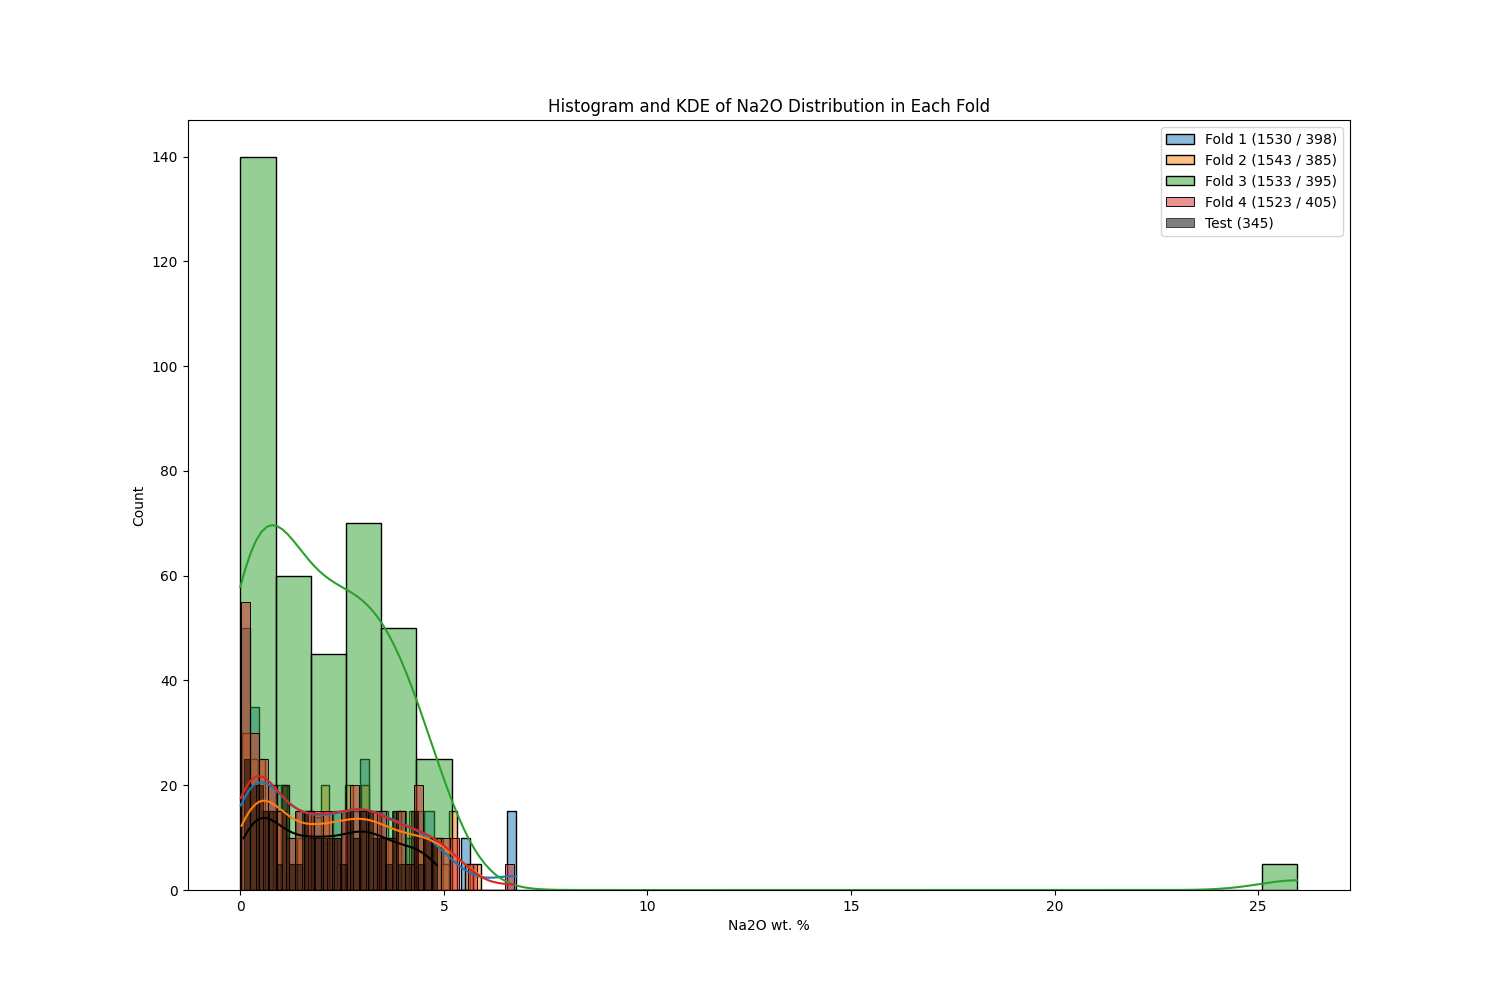
\includegraphics[width=\textwidth]{images/histogram_kde_plot.png}
    \caption{Combined Histogram and \gls{kde} of \ce{SiO_2} Distribution in Each Fold. The y-axis represents the count of samples per bin, and the x-axis represents \ce{SiO_2} concentration. The notation in the legend indicates the amount of instances in the training/validation sets.}
    \label{fig:histogram_kde_plot}
\end{figure*}

\begin{figure*}[h!]
    \centering
    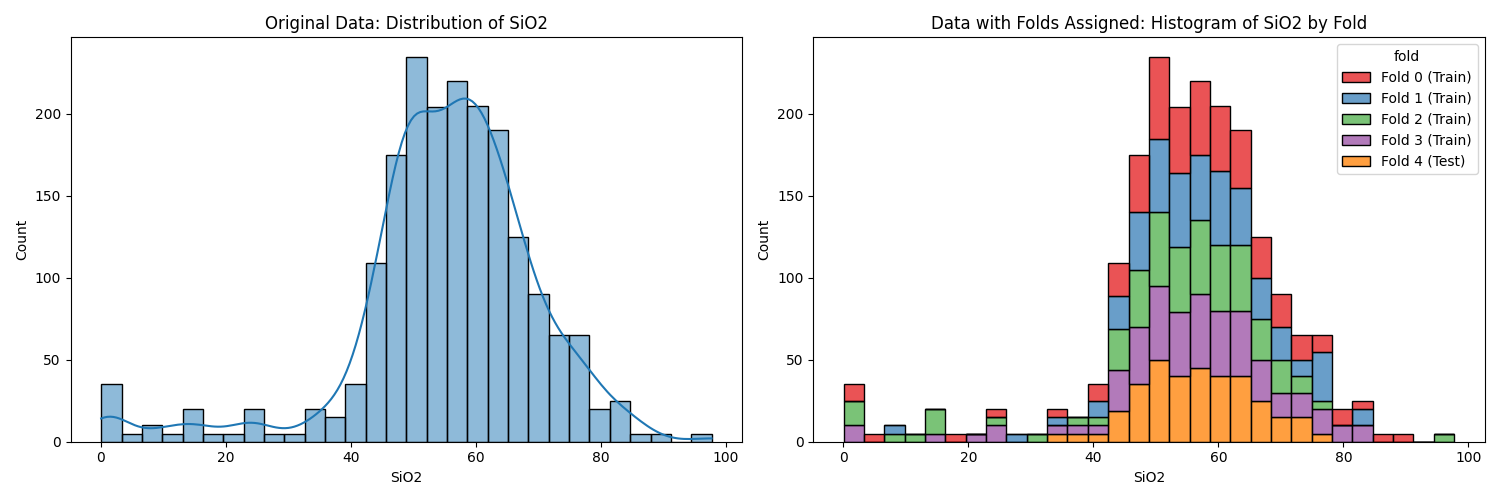
\includegraphics[width=\textwidth]{images/original_and_post_fold.png}
    \caption{Distribution of \ce{SiO_2} concentrations before and after fold assignment. The left plot shows the original distribution of \ce{SiO_2}, while the right plot shows the distribution with folds assigned, color-coded to indicate the different folds.}
    \label{fig:original_and_post_fold_plot}
\end{figure*}


To further validate our visual analysis, we can look at quantitative measures such as the means and standard deviations of \ce{SiO_2} concentrations across the folds and the overall dataset.

\begin{figure*}[htbp]
    \centering
    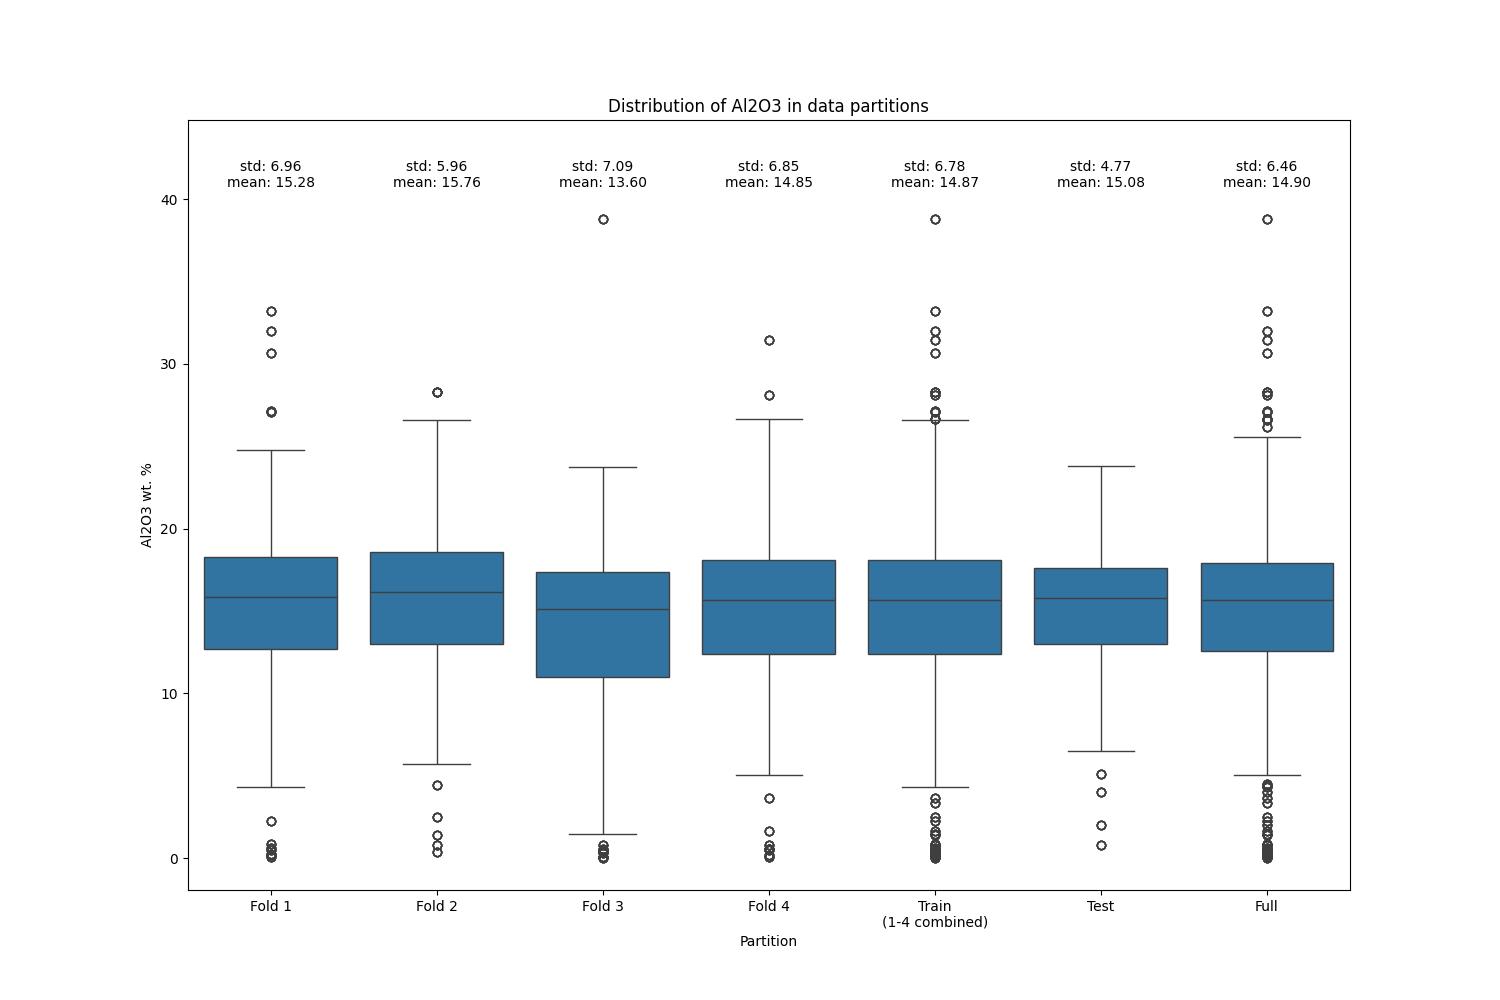
\includegraphics[width=\textwidth]{images/distribution_plot.png}
    \caption{Distribution of \ce{SiO_2} concentrations across cross-validation folds, training set, test set, and the entire dataset. The mean and standard deviation statistics for each partition are indicated figure.}
    \label{fig:siO2_distribution}
\end{figure*}

From Figure~\ref{fig:siO2_distribution}, it is evident that the means and standard deviations of \ce{SiO_2} concentrations for each fold, as well as the combined training set, are consistent with those of the full dataset.
This quantitative consistency supports the visual evidence that each training fold is representative of the entire dataset.
Furthermore, we can see that the standard deviation in the training sets is higher than the standard deviation in the test set, which is expected given the reassignment of extreme values to the training sets.

In conclusion, the visual and statistical analyses presented in this section confirm that our customized k-fold data partitioning procedure effectively maintains balanced and representative distributions across all folds.
This consistency is crucial for the robustness and generalizability of our models, as discussed in Section~\ref{subsec:validation_testing_procedures}.
The alignment between the visual evidence and the quantitative measures reinforces the reliability of our approach, ensuring that our models are well-equipped to perform accurately on unseen data.

\section{Discussion}\label{sec:discussion}
\section{Conclusion}\label{sec:conclusion}
\section{Future Work}\label{sec:future_work}
The findings of this study open several avenues for future research.
Firstly, for our data partitioning algorithm, described in Section~\ref{subsubsec:dataset_partitioning}, we noted that finding the optimal percentile value $p$ that minimizes extreme values in the test set, while maintaining its general representativeness, is important.
Future work should consider methods of quantitatively assesing and finding this value.
Such methods could include supplementary extreme value testing to the data partitioning algorithm, where after the primary evaluation, additional testing is conducted using a small, separate subset of extreme values to assess the model's performance on these critical cases.
For example, this could involve slightly reducing the percentile value $p$ and using the extreme values that fall within this reduced range to evaluate the model.

Another point of interest is limited data availability.
The small dataset size naturally limits the amount of how many extreme values are present.
These extreme values are an essential part of improving the model's generalizability, as they are the most challenging cases to predict.
Future work should investigate methods of augmenting the dataset with synthetic extreme value data to provide the model with more exposure to these cases during training.

Future work should also consider further experimentation with the choices of base estimators and meta-learners.
Our study highlighted that multiple model and preprocessor configurations perform well.
However, determining which configurations and meta-learner is optimal for a given oxide is a challenging task.
In this study, we used a simple grouping to ensure diversity in our base estimator selection, chosen from the top-performing configurations.
This approach could be improved upon by, for example, developing more advanced selection methods that consider the base estimators and meta-learners in conjunction. 